% Created 2016-08-17 Wed 14:38
\documentclass[tikz]{standalone}

\usepackage[utf8]{inputenc}
\usepackage[T1]{fontenc}
\usepackage{helvet}
\usepackage{../../templates/msc}

\renewcommand{\familydefault}{\sfdefault}

\tikzset{
every picture/.style={
line width=1pt
}}

\usepackage{tikz}
\author{Holger Karl}
\date{\today}
\title{}
  

\usetikzlibrary{chains,shapes.multipart}
\usetikzlibrary{shapes,calc}
\usetikzlibrary{automata,positioning}

\tikzset{
queue/.pic={
  \node (-open) at (0,0)  {}; 
  \node (-closed) at (3cm,0)  {}; 
  \draw[line width=1pt]
    (0,-0.5) -- ++(2.75cm,0) -- ++(0,1cm) -- ++(-2.75cm, 0cm);
    \foreach \Val in {1,...,#1} {
      \draw [rounded corners, fill=blue!20] (2.75cm-0.5cm*\Val-0.05cm,-0.45cm) rectangle (2.75cm-0.5cm*\Val+0.5cm-0.05cm, 0.45cm) node[pos=0.5] {\Val};
    }
  },
lqueue/.pic={
  \node (-open) at (0,0)  {}; 
  \node (-closed) at (-3cm,0)  {}; 
  \draw[line width=1pt]
    (0,-0.5) -- ++(-2.75cm,0) -- ++(0,1cm) -- ++(+2.75cm, 0cm);
    \foreach \Val in {1,...,#1} {
      \draw [rounded corners, fill=green!20] (-2.75cm+0.5cm*\Val-0.5cm+0.05cm,-0.45cm) rectangle (-2.75cm+0.5cm*\Val+0.05cm, 0.45cm) node[pos=0.5] (-\Val) {\Val};
    }
  },
    database/.style={
      cylinder,
      cylinder uses custom fill,
      cylinder body fill=yellow!50,
      cylinder end fill=yellow!50,
      shape border rotate=90,
      aspect=0.25,
      draw
    }
}

\begin{document}



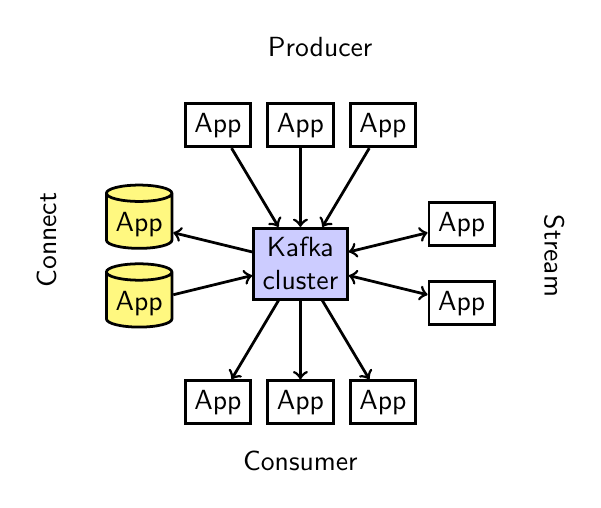
\begin{tikzpicture}% [line width=0.25mm]

\node [draw, align=center, fill=blue!20]  at (0,0) (k) {Kafka\\cluster};
\node [draw, above=of k] (a1)  {App}; 
\node [draw, above right =of k, xshift=-1cm]  (a2)  {App}; 
\node [draw, above left =of k, xshift=+1cm]  (a3)  {App}; 
\node [above of= a2, anchor=east] {Producer}; 

\node [draw, below left =of k, xshift=+1cm] (c1)   {App}; 
\node [draw, below  =of k]  (c2)  {App}; 
\node [draw, below right  =of k, xshift=-1cm] (c3)   {App}; 
\node [below = of c2, anchor=north, yshift=0.8cm] {Consumer}; 


\node [draw, right =of k, yshift=0.5cm] (s1)   {App}; 
\node [draw, right  =of k, yshift=-0.5cm] (s2)   {App}; 
\node [right = of s1, anchor=north, yshift=-0.4cm, rotate=270] {Stream}; 

\node [database, left =of k, yshift=0.5cm] (db1)   {App}; 
\node [database, left  =of k, yshift=-0.5cm] (db2)   {App}; 
\node [left = of db1, anchor=north, yshift=-0.2cm, rotate=90] {Connect}; 


\foreach \x in {a1,a2,a3} \draw [->]  (\x) -- (k); 
\foreach \x in {c1,c2,c3} \draw [->] (k) -- (\x); 
\foreach \x in {s1,s2} \draw [<->]  (\x) -- (k); 
\draw [->] (k) -- (db1); 
\draw [<-] (k) -- (db2); 


\end{tikzpicture}

% Kafka queues: 

% \end{document}

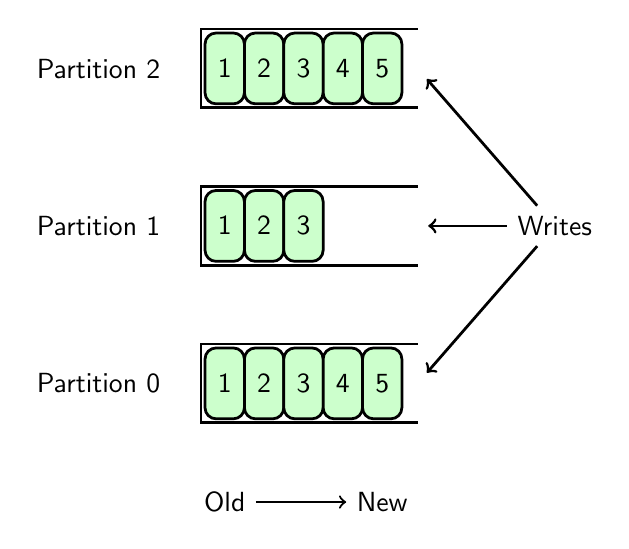
\begin{tikzpicture}
  
  \pic (q1) at (0,0) {lqueue=5}; 
  \pic (q2) at (0,2) {lqueue=3}; 
  \pic (q3) at (0,4) {lqueue=5};
  
  \node [left=of q1-closed, xshift=1cm] (p0) {Partition 0}; 
  \node [left=of q2-closed, xshift=1cm] (p1) {Partition 1}; 
  \node [left=of q3-closed, xshift=1cm] (p2) {Partition 2};

  \node (writes) [right= of q2-open] {Writes};

  \node (old) [below=of q1-1] {Old}; 
  \node (new)  at (q1-5|-old) {New}; 

  \draw [->] (writes) -- (q1-open); 
  \draw [->] (writes) -- (q2-open); 
  \draw [->] (writes) -- (q3-open); 

  \draw [thick, ->] (old) -- (new);
\end{tikzpicture}



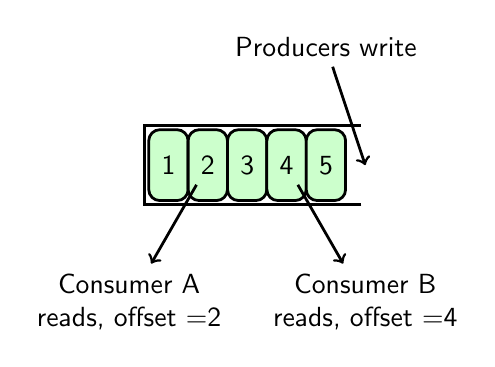
\begin{tikzpicture}
  \pic (q) at (0,0) {lqueue=5};
  
  \node [above=of q-5] (p)  {Producers write};
  \node [below=of q-2, xshift=-1cm, align=center] (ca) {Consumer A \\reads, offset =2};
  \node [below=of q-4, xshift=+1cm, align=center] (cb) {Consumer B \\reads, offset =4};
  
  \draw [->] (q-2) -- (ca); 
  \draw [->] (q-4) -- (cb); 

  \draw [->] (p) -- ($(q-5) + (0.5, 0)$);
\end{tikzpicture}

\begin{tikzpicture}

    \node [draw] (p0) {P0}; 
    \node [draw, right=of p0] (p3) {P3}; 

    \node [draw, right=of p3, xshift=0.5cm] (p1) {P1}; 
    \node [draw, right=of p1] (p2) {P2}; 

    \node [fit= (p0) (p3), draw] (s1)  {};
    \node [fit= (p1) (p2), draw] (s2) {};
    \node [above = 0cm of s1] (s1l) {Server 1}; 
    \node [above = 0cm of s2] (s2l) {Server 2}; 
    \node [fit= (s1) (s2) (s1l) (s2l), draw, dotted,
    label=above:{Cluster}] (kc) {};
    
    % -----------

    \node [draw] (c1) at (-1, -2) {C1}; 
    \node [draw, right=of c1] (c2) {C2}; 
    \node [draw, right=of c2] (c3) {C3}; 
    \node [draw, right=of c3] (c4) {C4}; 
    \node [draw, right=of c4] (c5) {C5}; 
    \node [draw, right=of c5] (c6) {C6}; 

    \node [fit= (c1) (c2), draw, dotted,
    label=below:{Group A}] (cga) {};

    \node [fit= (c3) (c4) (c5) (c6), draw, dotted,
    label=below:{Group B}] (cgb) {};

    %-------------

    \draw [->] (p0.south) -- (c1.north); 
    \draw [->] (p0.south) -- (c3.north); 
    \draw [->] (p3.south) -- (c1.north); 
    \draw [->] (p3.south) -- (c4.north); 

    \draw [->] (p1.south) -- (c2.north); 
    \draw [->] (p1.south) -- (c5.north); 
    \draw [->] (p2.south) -- (c2.north); 
    \draw [->] (p2.south) -- (c6.north); 


\end{tikzpicture}


% test picture to get the queues to work out right: 
% \begin{tikzpicture}
%   \pic (q1) at  (0,0) {queue=3} ; 

%   \pic (q2) at (0,2)   {lqueue=5};

%   \draw [->, thick] (q2-closed)  to[out=180,in=180]  (q1-open); 
%   \draw [->, thick, red] (q1-closed)  to[out=0,in=0] (q2-open); 
% \end{tikzpicture}

\end{document}

